\documentclass{article}

\usepackage{geometry}
\usepackage[T1]{fontenc}
\usepackage[utf8]{inputenc}
\usepackage{amssymb}
\usepackage{amsmath}
\usepackage{german}

\usepackage{tikz}

\usepackage{listings}
\usepackage{color}

\newcommand{\kreis}[1]{\unitlength1ex\begin{picture}(2.5,2.5)%
	\put(0.75,0.75){\circle{2.5}}\put(0.75,0.75){\makebox(0,0){#1}}\end{picture}}

\begin{document}
	
	\section{Rechenoperationen}
	\begin{enumerate}
		\item Baum besteht aus Knoten (Kreise) und Kanten (Pfeile)
		\item Kanten verbinden Knoten mit ihren Kind-Knoten
		\item jeder Knoten (außer der Wurzel) hat \underline{genau ein} Elternteil
		\item Knoten ohne Kinder heißen "'Blätter"' (leaf-nodes)
		\item Teilbaum
		\begin{enumerate}
			\item wähle beliebigen Knoten
			\item entferne temporär dessen Eltern-Kante
			\begin{enumerate}
				\item der Knoten wird temorär zu einer Wurzel
				\item dieser Knoten mit allen seinen Nachkommen bildet wieder seinen Baum - "' Teilbaum des Originalbaums"'
			\end{enumerate}
			\item Tiefe: Abstand des Knotens zur Wurzel
			\item 
		\end{enumerate}
	\end{enumerate}
	
	Infix-Notation: \\
	 $1+2+3*4/(1+5)-2$ \\ \\
	 Präfix-Notation: \\
	 $sub(add(add(1,2), div(mul(3,4), add(1,5))),2)$ \\ \\
	 
	 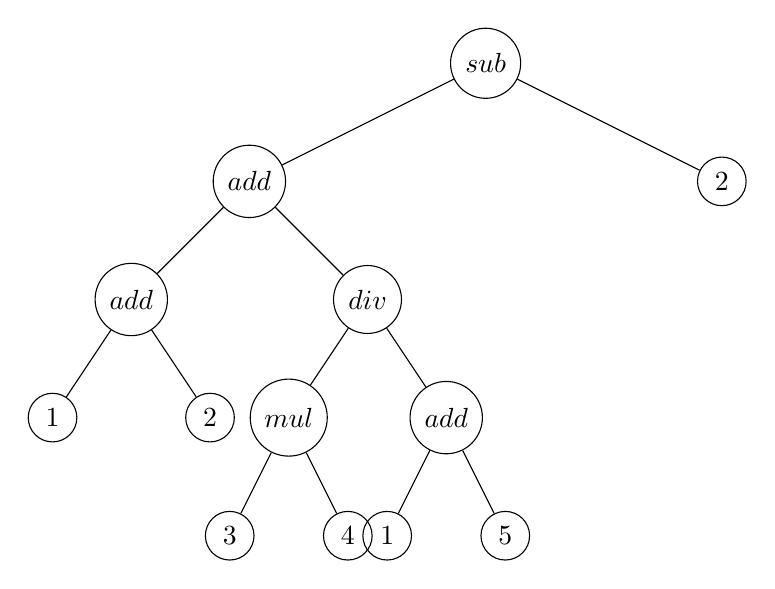
\begin{tikzpicture}[level/.style={sibling distance=60mm/#1}]
	 	
	 	\node [circle, draw] (z)  {$sub$}
	 	child {node [circle, draw] {$add$}
	 		child {node [circle, draw] {$add$}
	 			child{node [circle, draw] {$1$}}
	 			child{node [circle, draw] {$2$}}
	 		}
	 		child {node [circle, draw] {$div$}
	 			child{node [circle, draw] {$mul$}
	 				child {node [circle, draw] {$3$}}
	 				child {node [circle, draw] {$4$}}
	 			}
	 			child{node [circle, draw] {$add$}
	 				child {node [circle, draw] {$1$}}
	 				child {node [circle, draw] {$5$}}
	 			}
	 		}}
	 		child {node [circle, draw] {$2$}
	 		};
	 	\end{tikzpicture}
	 		
	\paragraph{Präfix Notation aus dem Baum rekonstruieren}
	 		
	 \begin{enumerate}
	 	\item Wenn die Wurzel ein Blatt ist, dann "'Drucke die Zahl"'
	 	\item sonst (Operator):
	 	\begin{enumerate}
	 		\item Drucke Funktionsnamen
	 		\item Drucke "'("'
	 		\item wiederhole ab $1)$ für das linke Kind
	 		\item Drucke "',"'
	 		\item wiederhole den Algorithmus ab $1)$ für das rechte Kind
	 		\item Drucke "')"'
	 	\end{enumerate}
	 \end{enumerate}
	
		Beachte Reihenfolge: Wurzel - Links - Rechts (Pre-Order Traversal)
		Ergebnis: \\
		$sub(add(add(1,2), div(mul(3,4), add(1,5))),2)$
		
		\paragraph{Definition: Rekursion}
		Rekursion meint Algorithmus für Teilproblem von vorn
		
		\paragraph{Infix Notation}
		
		\begin{enumerate}
			\item wie bei Präfix
			\item sonst
			\begin{enumerate}
				\item entfällt
				\item wie bei Präfix
				\item wie bei Präfix
				\item Drucke Operatorsymbol
				\item wie bei Präfix 
				\item wie bei Präfix
				\item wie bei Präfix
			\end{enumerate}
		\end{enumerate}
		Beachte Reihenfolge: Links - Wurzel - Rechts (In-Order Traversal) \newline
		
		Ergebnis: \\
		$(((1 + 2) + ((3 * 4)/(1 + 5))) + 2)$
		
		\paragraph{Berechne den Wert mit Substitutionsmethode}
		\begin{enumerate}
			\item Wenn Wurzel ein Blatt hat, gib die Zahl zurück
			\item sonst
			\begin{enumerate}
				\item entfällt
				\item entfällt
				\item wiederhole ab $1)$ für linken Teilbaum und speichere Ergebnis als "'left-result"'
				\item entfällt
				\item wiederhole ab $1)$ für rechten Teilbaum, speichere Ergebnis als "'right-result"'
				\item berechne $fkt_name(left-result, right-result)$ und gib Ergebnis zurück
			\end{enumerate}
		\end{enumerate}
		Beachte Reihenfolge: Links - Rechts - Wurzel (Post-Order Traversal)
		
		\begin{align*}
		&  	sub(add(add(1,2), div(mul(3,4), add(1,5))),2) \\
		= & \, sub(add(add(1,2), div(12, 6)),2) \\
		= & \, sub(add(3,2)2) \\
		= & \, sub(5,2) \\
		= & \, 3
		\end{align*}
		
		\section{Maschinensprache}
		\begin{itemize}
			\item optimiert für die Hardware (viele verschiedene)
			\item Gegensatz: höhere Programmiersprache ($C++$) ist optimiert für Programmierer
			\item Compiler oder Interpreter übersetzen Hoch- in Maschinensprache 
		\end{itemize}
		
		\paragraph{Vorgang des Übersetzens}
		\begin{enumerate}
			\item Eingaben (und Zwischenergebnisse) werden in Speicherzellen abgelegt $ \Rightarrow$ jeder Knoten im Baum bekommt eine Speicherzelle (Maschinensprache: durchnumeriert ; Hochsprache: sprechende Namen)
			\item Speicherzellen für die Eingaben $\underline{initialisieren}$ ; Notation: SpZ $\leftarrow$ Wert
			\item Rechenoperationen in der Reihenfolge des Substitutionsmodells ausführen und in der jeweiligen Speicherzelle speichern ; Notation: SpZ\_Ergebnis $\leftarrow$ fkt\_name SpZ\_Arg1 SpZ\_Arg2
			\item alles in Zahlencode umwandeln
			\begin{itemize}
				\item Funktionsname $\Rightarrow$ Opcodes
				\item Speicherzellen: nur die Nummer
				\item Werte sind schon Zahlen
				\item Notation: Opcode \quad Ziel SpZ \quad SpZ\_Arg1 \quad SpZ\_Arg2 oder Opcode \quad Ziel SpZ \quad Initialwert
			\end{itemize}
		\end{enumerate}
	
	\section{funktionale Programmierung}
	(alles durch Funktionsaufrufe ausführen)
	
	\begin{enumerate}
		\item bei Maschinensprache wurden Zwischenergebnisse in Speicherzellen abgelegt
		\item das ist auch in der funktionalen Programm. eine gute Idee
		\begin{enumerate}
			\item Speicherzellen werden durch Namen (vom Programmierer vergeben) unterschieden
			\item Beispiel: Lösen einer quadratischen Gleichung: $ax^2+bx+c =0$, finde $x_{1/2}$
					$\Rightarrow x^2-px+q =0 \quad mit \quad p = -\frac{b}{2a}, q = \frac{c}{a}$
					$\Rightarrow x_1 = -\frac{b}{2a} + \sqrt{(-\frac{b}{2a}^2 - \frac{c}{a})} \\ \Leftarrow allgemein: x_{1/2} = p \pm \sqrt{p^2-q}$
			\item Präfix: \\ $x_1 \leftarrow add(div(div(b,a),-2), sqrt(sub(mul(div(div(b,a),-2), div(div(b,a), -2)), div(c,a))))$ \\
					mit Zwischenergebnissen und Infix-Notation: $p \leftarrow b/c/-2 \quad $oder$ \quad p \leftarrow -0,5*b/a \quad q \leftarrow c/a$ \\ $discriminant \leftarrow sqrt(p*P-q)$ \\
					$x_{1/2} \leftarrow p \pm discriminant$
		\end{enumerate}
		\item zwei Vorteile:
		\begin{enumerate}
			\item lesbar
			\item redundante Berechnung verschieden \\ Beachte: In der funktionalen Programmierung können die Speicherzellen nach der Initialisierung \underline{nicht} mehr verändert werden
			\item Speicherzellen mit Namen sind nützlich, um Argumente an Funktionen zu übergeben $\Rightarrow$ Definition eigener Funktionen \\
			Bsp: 
			\framebox{function sq(x) \\
												\{
												return x*x
												\} }
		\end{enumerate}
	\end{enumerate}
	
	\section{funktionale Programmierung in C++}
	
	\begin{enumerate}
		\item in C++ hat jede Speicherzelle einen \underline{Typ} (legt Größe und Bedeutung der Speicherzelle fest) \\
		wichtigste Typen: \grqq int\grqq  für ganze Zahlen, \grqq double\grqq  für reelle Zahlen, \grqq std::string\grqq  für Text \\ zugehörige Literale (Konstanten): 12, -3 (int) \quad -1.02 , 1.2e-4 (double) \quad \grqq text text \grqq (string)
		\item Die Initialisierung wird geschrieben als
		\begin{lstlisting}[tabsize =2]
			type_name spz_name = initialwert
		\end{lstlisting}
		Bsp:
		\begin{lstlisting}[tabsize = 2]
			double a = 10
			std::cout << "x_1" << x_1 << "\n" ;
		\end{lstlisting} 
		\item eigene Funktion in $C++$: 

			\begin{lstlisting}[tabsize = 2]
			type_ergebnis funktionsname (typ_arg1 name_arg1, typ_arg2 name_arg2)
			{
				<code>
				return ergebnis;
			}
			\end{lstlisting}
			
		\item zwei Funktionen mit gleichem Namen, aber unterschiedlichen Typen dürfen in C++ gleichzeitig definiert sein (\grqq overloading\grqq) \\ $\Rightarrow$ C++ wählt \underline{automatisch} die richtige Variante anhand des Argumenttypes (\grqq overload resolution\grqq)
		
		\item jedes $C++$ -Programm muss \underline{genau eine} Funktion names \grqq main\grqq haben: Dort beginnt die Programm-Ausführung \\
		Bsp: \\
		\fbox{\centering int main() \{ <code> \quad return 0 (erfolgreich abgearbeitet)\}}
		
		\item Regel von $C++$ für erlaubte Namen (Speicherzelle \& Funktion):
		\begin{enumerate}
			\item erste Zeichen: Klein- oder Großbuchstaben des englischen Alphabets oder \_
			\item optional: weitere Zeichen: wie erstes Zeichen oder Ziffern 0 \dots 9
		\end{enumerate}
		
		\item vordefinierte Funktionen in $C++$
		\begin{enumerate}
			\item eingebaute Funktionen (immer vorhanden) z.B. Infix Operatoren
			\item Funktionen der Standardbibliothek (Programmierer muss sie explizit auffordern)
			\begin{enumerate}
				\item z.B. algebraische Funtionen beginnend mit std::\dots
				\item sind in Module geordnet, z.B. cmath $\widehat{=}$ \, algebraische Funktionen, iostream $\widehat{=}$ \, Ausgabe, z.B. std::cout
				\item Um ein Modul zu benutzen, muss man zuerst (am Anfang des Programms) sein Inhaltsverzeichnis importieren \\
				\frame{\centering \#include <module\_name>} sprich \grqq Header inkludieren\grqq \\
				 \\
			\end{enumerate}
		\end{enumerate}
	\end{enumerate}
	
	\begin{lstlisting}
	# include <iostream> 
	# include <string> 
	
	int main() {
	
	std::cout <<  "Hello" << "\n";
	std::string >> ausgabe = "mein erstes Programm"
	std::cout << ausgabe;
	
	return 0
	}
	\end{lstlisting}
	
	\paragraph{Overloading der arithmetischen Operationen}
	
	\begin{lstlisting}
		int a = 3;
		int b = 4;
		int c = a * b;
		double x = 3.0;
		double y = 4.0;
		double z = x * y;
	\end{lstlisting}
	$3.0 * 4 \quad \Rightarrow \quad$ automatische Umwandlung in höheren Typ, hier: \grqq double\grqq $\Rightarrow$ wird als $3.0 * 4.0$ ausgeführt \\
	
	\paragraph{Interger-Division in $C++$}
	
	Konsequenzen:
	\begin{enumerate}
		\item Division unterscheidet sich nach dem Datentypen: $(-12)/5 \Rightarrow -2 \neq -2.4 \Leftarrow (-12.0/5.0)$
		\item negative Ereignisse werden aufgerund, positive abgerundet (truncating division) \\
				d.h. Nachkommstellen abschneiden, d.h. Richtung Null runden
		\item Gegensatz (z.B. zu Python): floor division $\widehat{=}$ wird immer abgerundet
		\item Divisionsrest: 
			\end{enumerate}
		\begin{lstlisting} [tabsize = 2]
			int a = ...;
			int b = ...;
			int q = a/b;
			(a/b)*b = q * b
		\end{lstlisting}
		ist im allgemeinen \underline{ungleich} $a$ $\Rightarrow$ 
		\begin{lstlisting} [tabsize = 2]
			int rest = a = q*b;
		\end{lstlisting}
		\begin{enumerate}
		\item wenn Division aufgeht $\Rightarrow$ rest = 0 , sonst $\neq 0$
		\item Invariante: 
		\begin{lstlisting} [tabsize = 2]
			(a/b) * b + rest = a
			
			int rest1 = a % b;  // aequivalent: a-(b/a)*b
		\end{lstlisting}
	\end{enumerate}
	
	\paragraph{Anwendung}
	
	Wochentag für beliebiges Datum bestimmen:
	gegeben: $d,m,y$ , gesucht: $w \in \{0,\dots , b\}$ \\
		int weekday(int d, int w, int y) {}  ; weekday(10,11,2016) $\Rightarrow$ 3 (Donnerstag)
		
		Teilprobleme
		\begin{enumerate}
				\item finde den Wochentag vom 1. Januar y
				\item finde den Abstand vom (d,m,y) zum (1,1,y)
				\item setze beides zusammen \\

		\end{enumerate}
		
	Schaltjahresregel: y ist Schaltjahr, wenn:
	\begin{enumerate}
		\item y durch 4 teilbar, aber nicht durch 100 $\Rightarrow$ 2004, 2006, nicht 2100
		\item y durch 400 teilbar $\Rightarrow$ 2000 \\ \\
		 $\Rightarrow$ 400-Jahres-Zyklus der Regeln: nach 400 Jahren beginnt die Schaltjahresregel von vorn
 	\end{enumerate}
 	
 	\begin{itemize}
 		\item Beobachtung: der 1.1.2001 ist der erste Tag eines neuen Zyklus und war Montag
 		\item die Anzahl der Tage vom 1.1.y zum 1.1.2001 ist: \\
 		$z = y - 2001 \quad \triangle = 365 * z + z/4 - z/100 + z/400$
 		\item floor division ist wichtig, wenn $z<0$, z.B. $y = 2000\, , z=-1$
 	\end{itemize}
 	
 	zu \kreis{2}: d.m. ist der x-te Tag im Jahr mit: \\
	 	\begin{itemize}
			\item kein Schaltjahr
				\begin{enumerate}
					\item $m=1 \Rightarrow d$
					\item $m=2 \Rightarrow d+31$
					\item $m=3 \Rightarrow d+59$
					\item $m=4 \Rightarrow d+90$
					\item $m=5 \Rightarrow d+120$
					\item $m>2 \Rightarrow d+59+(153*m-457)/5$
				\end{enumerate}
			\item Schaltjahr
			\begin{enumerate}
				\item $m=1 \Rightarrow d$
				\item $m=2 \Rightarrow d+31$
				\item $m=3 \Rightarrow d+60$
				\item $m=4 \Rightarrow d+91$
				\item $m=5 \Rightarrow d+121$
				\item $m>2 \Rightarrow d+60+(153*m-457)/5$
			\end{enumerate}
		
		zu \kreis{3}: Wochentag von d, m, y:
		\begin{lstlisting} [tabsize = 2]
			w = (w_11y + x - 1) mod 7
		\end{lstlisting}
	 	\end{itemize}
	 	
	 	\paragraph{Bedingungen}
	 	\begin{itemize}
	 		\item Bei den meisten Algorithmen ist die Reihenfolge der Schritte \underline{nicht} fix, sondern hängt von den Eingabedaten ab
	 		\item Beispiel: Auswahl der Offset $d \rightarrow x$ hängt von m ab \\
	 		dafür die Funktion:
	 		\begin{lstlisting}
	 			cond ( bedingung , resultat_wenn_wahr , resultat_wenn_falsch )
	 		\end{lstlisting}
	 		\item kanonische Beispiele: Absolutbetrag, Vorzeichenfunktion
	 	\end{itemize}
	 	
	 	Bedingungen programmieren:
	 	\begin{itemize}
	 		\item relationale Operatoren: Vergleich von zwei Argumenten \\ $< , > , <= , >= , !=$
	 		\item logische Operatoren: Verknüpfen von mehreren Bedingungen \\
		 		$ \&\& (und), || (oder), != (nicht)$
		 	\item in $C++$ gibt es \underline{keine} Prefix-Variante für die \textit{cond()}-Funktion, aber eine Infix-Variante:
		 	\begin{lstlisting} [tabsize = 2]
				(bedingung) ? erg_wenn_wahr : erg_wenn_falsch
				
				int abs (int x) {
					return (x >= 0) ? x : -x;
				}
				double abs (double x) {
					return (x >= 0.0) ? x : -x;
				}
				int sign (int x) {
					return (x == 0) ? 0 : ((x > 0) ? 1 : -1);
				}
		 	\end{lstlisting}
	 	\end{itemize}
	 	
	 	\paragraph{Rekursion}
	 	
	 	bedeutet: eine Funktion ruft sich selbst auf (evtl. indirekt)
	 	\begin{itemize}
	 		\item kanonisches Beispiel: Fakultätsfunktion $k! = 1 \cdot 2 \cdot \dots (k-1) \cdot k$
	 		\item in $C++$ (rekursive Definition)
	 		\begin{lstlisting} [tabsize = 2]
	 			int fakultaet (int k) {
		 			return (k == 0) ? 1 : k * fakultaet(k-1) ;
	 			}
	 		\end{lstlisting}
	 		\item wichtige Eigenschaften:
	 		\begin{itemize}
	 			\item jede rekursive Funktion muss mindestens einen nicht-rekursiven Zweig enthalten, der nach endlich vielen rekursiven Aufrufen erreicht wird \grqq Rekursionsabschluss\grqq - sonst: Endlosrekursion (Absturz)
				\item bei jedem Aufruf werden dem Namen der Dateenelemente (Argumente \& Zwischenergebnisse) \underline{neue} Speicherzellen zugeordnet \\
				\textit{fakultaet(3)} $\rightarrow \textit{fakultaet(2)} \rightarrow \textit{fakultaet(1)} \rightarrow \textit{fakultaet(0)} \quad \Rightarrow $ \\
				$\textit{return 3*fakultaet(2)} \leftarrow \textit{return 2*fakultaet(1)} \leftarrow \textit{return 1*fakultaet(0)} \leftarrow \textit{return 1}$
				
	 		\end{itemize}
	 	\end{itemize}
	 	
	 	\paragraph{Von der funktionalen zur prozeduralen Programmierung}
	 	\begin{itemize}
	 		\item Eigenschaften der FP:
	 		\begin{itemize}
	 			\item alle Berechnungen durch Funktionsaufrufe, Ergebnis ist Rückgabe
	 			\item Ergebnis hängt nur von den Werten der Funktions-Argumente ab, nicht von externen Faktoren (\textit{referentielle Integrität})
	 			\item Speicherzellen für Zwischenergebnisse/Argumente können nach der Initialisierung nicht geändert werden (\textit{write once})
	 			\item Möglichkeit der rekursiven Funktionsaufrufe (jeder Aufruf bekommt eigene Speicherzellen)
	 		\end{itemize}
	 		\item Vorteile:
	 		\begin{itemize}
	 			\item natürliche Ausdrucksweise für arithmetische und algebraische Funktionalität (\textit{Taschenrechner})
	 			\item einfache Auswertung durch Substitutionsmodell - Auswertungsreihenfolge nach Post-Order
	 			\item mathematisch gut formalisierbar $\Rightarrow$ Korrektheitsbeweise (besonders bei Parallelverarbeitung)
	 			\item Rekursion ist mächtig und natürlich für bestimmte Probleme (z.B. Fakultät)
	 		\end{itemize}
	 		\item Nachteile:
	 		\begin{itemize}
	 			\item viele Probleme lassen sich anders natürlicher ausdrücken (z.B. Rekursion vs. Iteration)
	 			\item setzt unendlich viel Speicher vorraus ($\Rightarrow$ Memory management notwendig $\Rightarrow$ später)
	 			\item Entitäten, die sich zeitlich verändern schwer modellierbar, teilweise unnatürlich
	 		\end{itemize}
	 		\item Korrolar: Man kann keine externen Resourcen (z.B. die Console/Drucker, Bildschirm) ansprechen (weil zeitlich veränderlich) \\ "'keine Seiteneffekte"'
	 		\item Lösung: Einführung einer Multi-Paradigmensprachen, z.B. Kombination von funktionaler mit \underline{prozeduraler} Programmierung
	 	\end{itemize}
	 	
	 	
	 	\section{Prozeduale Programmierung}
 	
 	\begin{itemize}
 		\item Kennzeichen:
 		\begin{itemize}
 			\item Prozeduren - Funktionen, die nichts zurückgeben, haben nur Seiteneffekte \\ \underline{Bsp:} auf Konsole ausgeben
 			\begin{lstlisting} [tabsize = 2]
 				std::cout << "Hello World \n";  // Infix
 				operator << (std::cout, "Hello \nLeftarrow"); // Praefix notation
 			\end{lstlisting}
 			\item Prozeduren in $C++$:
 			\begin{enumerate}
 				\item Funktion, die \textit{void} zurückgibt (Pseudotyp nur "'nichts"')
 				\item Returnwert ignorieren
 			\end{enumerate}
 			\item Anweisen zur Steuerung des Programmablaufs (z.B. \textit{if / else})
 			\begin{lstlisting} [tabsize = 2]
	 			// funktional:
	 			int abs (int x) {
		 			return (x>=0) ? x : -x ;
	 			}
	 			
	 			// prozedural
	 			int abs (int x) {
		 			if (x >= 0) {
			 			return x;
		 			} else {
			 			return -x;
		 			}
	 			}
 			\end{lstlisting}
 		\end{itemize}
 		\item Zuweisung:
 		\begin{itemize}
 			\item Speicherzellen können nachträglich verändert werden "'\textit{read-work}"'
 			\begin{lstlisting} [tabsize = 2]
	 			// prozedural
 				int foo (int x) {
	 				int y =2;
	 				int z1 = x * y;  // z1 = 6
	 				y = 5;
	 				int z2 = x * y;  // z2 = 15
	 				return z1 + z2;
 				}
 				// write once
 				typ const name = wert
 				
 				// funktional 
 				int foo (int x) {
	 				int y = 2;
	 				int z1 = x * y;  // z1 = 6
	 				int y2 = 5;
	 				int z2 = x * y2;  // z2 = 15
	 				return z1 + z2;
 				}

 			\end{lstlisting}
 		\end{itemize}
 		\item $\Rightarrow$ Folgen:
 		\begin{itemize}
 			\item mächtiger, aber ermöglicht völlig neue Bugs $\Rightarrow$ Erhöhte Aufmerksamkeit beim Programmieren
 			\item die Reihenfolge der Ausführung ist viel kritischer als beim Substitutionsmodell
 			\item der Programmierer muss immer ein mentales Bild des aktuellen Systemzustands haben
 		\end{itemize}
 	\end{itemize}
	
	\paragraph{Schleifen}
	 der gleiche Code soll oft wiederholt werden \\ \\
	 
	 \begin{lstlisting} [tabsize = 2]
	 	while (bedingung) {
		 	... // code wird ausgefuehrt, solange bedingung "true" ist
	 	}
	 \end{lstlisting}
	 \underline{Bsp:} Zahlen von 0-2 ausgeben)
	 \begin{lstlisting} [tabsize = 2]
		 int counter = 0;
		 while (counter < 3) {
			 std::cout << counter << "\n";
			 counter = counter +1;
		 }
	 \end{lstlisting}
	 
	 \begin{tabular} {c|c|c}
	 	counter & Bedingung & Ausgabe \\
	 	\hline
	 	0 & true & 0 \\
	 	1 & true & 1 \\
	 	2 & true & 2 \\
	 	3 & false & $\varnothing$
	 \end{tabular}
	 
	\begin{itemize}
		\item $C++$ beginnt mit der Zählung meist bei $0$ "'\textit{zero-based}"'
		\item vergisst man Inkrementierung counter = counter +1 $\Rightarrow$ Bedingung immer true $\Rightarrow$ Endlosschleife $\Rightarrow$ Bug
		\item drei äquivalente Schreibweisen für Implementierung:
		\begin{lstlisting} [tabsize = 2]
			counter = counter + 1;  // assignment
			counter += 1;  // add-assignment
			++ counter;  // pre-increment
		\end{lstlisting}
	\end{itemize}
	
	\paragraph{Anwendung: Wurzelberechnung}
	
	Ziel: \text{double sqrt (double y)}
	Methode: \underline{iterative Verbesserung} mittels Newtonverfahren
	\begin{lstlisting} [tabsize = 2]
		initial guess  x(0) bei t=0 geraten
		while not_good_enough(x(t)) {
			update x(t+1) from x(t)
			t = t+1
		}
	\end{lstlisting}
	Newtonverfahren: finde Nullstelle einer gegebenen Funktion $f(x)$, d.h. suche $x^\star$, sodass $f(x^\star)=0$ oder $|f(x^\star)| < \epsilon$
	\begin{enumerate}
		\item Taylorreihe von $f(x)$: $f(x+\triangle) \approx f(x) + f'(x) \cdot \triangle + \dots$
		\item $0 = f(x^\star) \approx f(x) + f'(x) \cdot \triangle = 0 \Rightarrow \triangle = -\frac{f(x)}{f'(x)}$
		\item Iterationsvorschrift: $x^{(t+1)} = x^{(t)} - \frac{f(x^{(t)}}{f'(x^{(t)}}$
		\item Anwendung auf WurzeL: setze $f(x) = x^2 -y \Rightarrow mit f(x^\star) =0 gilt (x^\star)^2 -y=0$
		\item Iterationsvorschrift: $x^{(t+1)} = x^{(t)} - \frac{(x^{(t)})^2 -y}{2 x^{(t)}} = \frac{(x^{(t)})^2 + y}{2 x^{(t)}}$ \\
		$ x^{(t+1)} = \frac{x^{(t)} + \frac{y}{x^{(t)}}}{2}$ mit $ x^\star = \sqrt{y} \Rightarrow x^{(t+1)} = \sqrt{y}$
		
	\end{enumerate}
	\begin{lstlisting} [tabsize = 2]
		double sqrt (double y) {
			if (y<0.0) {
				std::cout << "Wurzel aus negativer Zahl \n";
				return -1.0;
			}
			if (y == 0.0) {
				return 0.0;
			}
			double x = y;  // initial guess
			double epsilon = 1e-15 * y;  // double Genauigkeit
			
			while (abs(x*x-y) > epsilon) {
				x = (x + y/x) / 2.0 ;
			}
			return x;
		}
	\end{lstlisting}
	
\end{document}